%!TEX root = ../main/main.tex
\section{Data management view} % (fold)
\label{sec:data_management}
This section focuses on policies and data storing management.\\
\subsection{Data Policy} % (fold)
\label{sub:data_policy}
\subsubsection{Automatic data elimination} % (fold)
\label{ssub:data_elimination}
Data about \emph{Users} and \emph{Taxi Drivers} is never automatically eliminated from the system.\\
However rides log are kept for 12 months to save storage space and to speed up queries.
% subsubsection data_elimination (end)
\subsubsection{Data caching policy} % (fold)
\label{ssub:data_caching}
In order to reduce the load on the \emph{Server} and to speed up user's query response, all the data that does not change frequently (like the user's profile data) is saved locally on the device and reloaded only when a modification of the profile occurs.

% subsubsection data_caching (end)
\subsection{Data storing} % (fold)
Here is a presentation of the data base schema that will have to be used:

\label{sub:data_storing}
\begin{figure}[h!t]
\caption{ER Diagram}
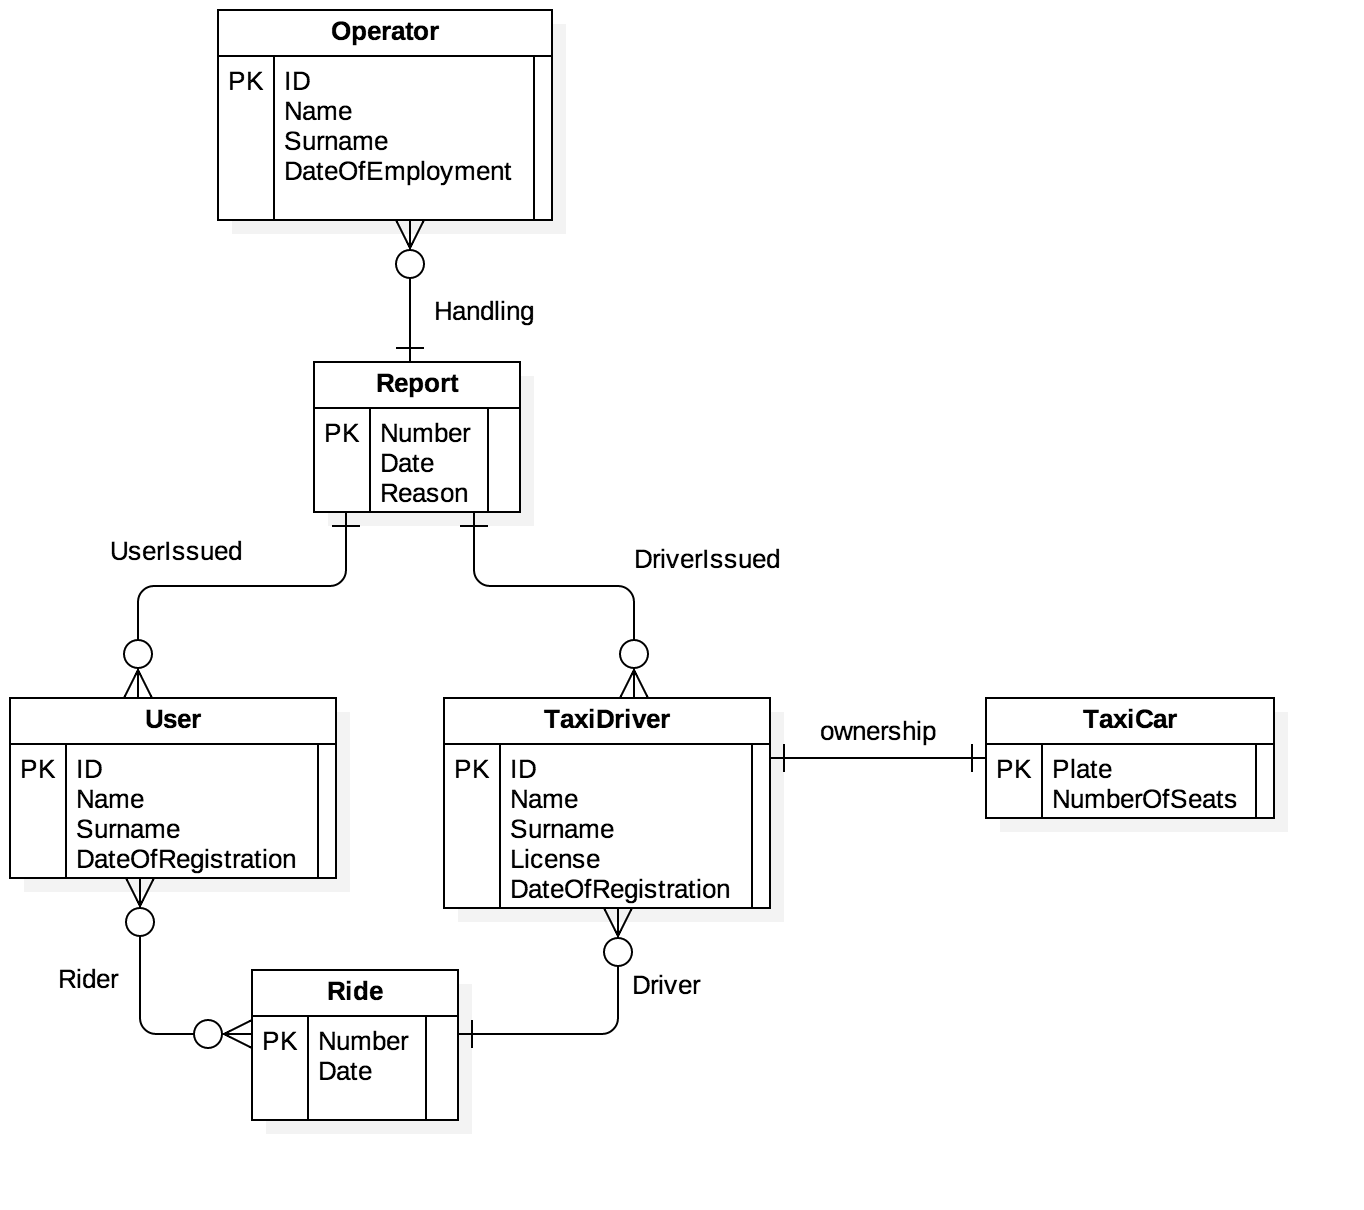
\includegraphics[width=\textwidth]{diagram/png/ERD}
\centering
\end{figure}
\newpage

% subsection data_storing (end)
